% Provenance (never printed): old premiere S material on subduction (Wadati-Benioff
% planes, density of the old lithosphere, slab pull, transformation of the slab at
% depth: blueschist and eclogite; anatomy of an active margin). Sections from
% figdata/grade-11/slab_sections.py (USGS ComCat M >= 6 1976-2025, PB2002 steps,
% Seton 2020 ages); plate speeds from plate_velocities.py (NNR-MORVEL56 RMS).
% Metamorphism is defined in g12.03, the volcanic arc in g12.04: named only here.
\chapter{نطاقات الاندساس}\label{ch:g11:subduction-zones}

تحت جزر تونغا، في جنوب غرب المحيط الهادئ، تهتز الأرض على أعماق
تفوق أي مكان آخر. فمن بين سبعة آلاف زلزال بقدر
6 فأكثر سُجلت في العالم بين 1976 و2025، وقع أعمقها على عمق
\qty{688}{km}، ويضم المقطع العرضي عبر تونغا في هذا الفصل أحداثًا يصل عمقها
إلى نحو \qty{671}{km}. على هذه الأعماق يكون الصخر ساخنًا وتحت ضغط
هائل؛ فكان ينبغي أن ينساب ببطء، \omterm{def:g11:lithosphere-asthenosphere:lithosphere}{كالغلاف اللدن}، لا أن ينكسر. ومع ذلك
ينكسر. يشرح هذا الفصل ما الذي يوجد هناك لينكسر: \omterm{def:g11:subduction-zones:slab}{لوح} من قاع محيطي
بارد، يغوص عائدًا إلى الوشاح.
% ledger: data:usgs-comcat (catalogue_maxdepth 688; tonga_maxdepth 670.8, slab_sections.py)

\begin{recall}
عند الحد المتقارب تتحرك صفيحتان إحداهما نحو الأخرى؛ وتحفّ خنادق عميقة
ببعض هذه الحدود (الكتاب 1، الصفان 7 و8). ويقيس قدر الزلزال
حجمه، والزلزال تحت البحر قد يولّد تسونامي
(الكتاب 1، الصف 7). وسرعة صفيحة بالنسبة إلى أخرى هي
فرق سرعتيهما (\cref{ch:g11:plate-motions}). ويغوص قاع المحيط
كلما تقدم في العمر، وبعد نحو 60 مليون سنة يصير غلافه الصخري، الذي يبلغ سمكه نحو
\qty{100}{km}، أكثف من \omterm{def:g11:lithosphere-asthenosphere:lithosphere}{الغلاف اللدن} الذي تحته
(\cref{ch:g11:ocean-ridges}). وتُظهر الموجات الزلزالية تغيرًا حادًا في الوشاح
على عمق نحو \qty{670}{km} (\cref{ch:g11:seismic-structure}). والصخر المتحول
صخر تحوّل وهو في الحالة الصلبة (الكتاب 1، الصف 6).
\end{recall}
% ledger: data:prem (670 km), ps77:depth-age

\section{الخنادق ونطاقات الزلازل المائلة}

معظم الزلازل ضحلة: ففي فهرس الزلازل التي قدرها 6 فأكثر منذ
1976، لا يزيد عمق إلا زلزال واحد من كل خمسة تقريبًا على \qty{70}{km}، وزلزال واحد من كل خمسة عشر
على \qty{300}{km}. وتبيّن الخريطة أدناه مواضع الزلازل العميقة.
% values (slab_sections.py): frac_deeper_70 0.21, frac_deeper_300 0.069; data:usgs-comcat

\begin{omfigure}
\begin{tikzpicture}
\begin{axis}[ommap, width=\linewidth, xtick={-180,-90,...,180}, ytick={-60,0,60},
  legend style={font=\scriptsize, at={(0.5,-0.13)}, anchor=north, legend columns=3,
    /tikz/every even column/.append style={column sep=6pt}}]
\addplot[fill=omLithAlluv, draw=black!45, line width=0.2pt, forget plot] table {figdata/out/shared-geo-land.dat};
\addplot[black!70, line width=0.5pt, forget plot] table {figdata/out/shared-geo-school-subduction.dat};
\addplot[fill=black!70, draw=none, forget plot] table {figdata/out/shared-geo-school-teeth.dat};
% computed in figdata/grade-11/slab_sections.py; ledger: data:usgs-comcat, data:pb2002
\addplot[only marks, mark=*, mark size=0.55pt, black!45] table[x=lon, y=lat] {figdata/out/grade-11-slab_sections-world-shallow.dat};
\addplot[only marks, mark=*, mark size=0.8pt, omProp] table[x=lon, y=lat] {figdata/out/grade-11-slab_sections-world-mid.dat};
\addplot[only marks, mark=*, mark size=1.1pt, omThm] table[x=lon, y=lat] {figdata/out/grade-11-slab_sections-world-deep.dat};
\legend{{\foreignlanguage{arabic}{أقل عمقًا من \babelsublr{\qty{70}{km}}}}, {\foreignlanguage{arabic}{من 70 إلى \babelsublr{\qty{300}{km}}}}, {\foreignlanguage{arabic}{أعمق من \babelsublr{\qty{300}{km}}}}}
\end{axis}
\end{tikzpicture}

{\small الزلازل التي قدرها 6.5 فأكثر، 1976--2025 (2192 حدثًا)،
ملونة بحسب العمق، مع الخنادق (الخط الأسود، والمثلثات على الصفيحة
الراكبة). ولا تقع الزلازل المتوسطة العمق والعميقة إلا على امتداد بعض الخنادق،
ودائمًا على جانب الصفيحة الراكبة. البيانات: فهرس الزلازل لهيئة المسح الجيولوجي الأمريكية؛
حدود الصفائح لبيرد (2003)؛ اليابسة من Natural Earth.}
\end{omfigure}
% values: world_n_m65 2192, world_deep_n 197 (slab_sections.py)

الزلازل العميقة ليست مبعثرة: فهي تتبع خنادق
غرب المحيط الهادئ، من كامتشاتكا إلى اليابان وجزر ماريانا وإندونيسيا وتونغا،
والخندق الممتد على امتداد الساحل الغربي لأمريكا الجنوبية؛ وهي تقع دائمًا على
جانب واحد من الخندق، تحت الصفيحة التي لا تغوص.

\begin{definition}[الاندساس؛ نطاق الاندساس]\label{def:g11:subduction-zones:subduction}
\emph{الاندساس}\index{اندساس} هو غوص صفيحة من \omterm{def:g11:ocean-ridges:oceanic-lithosphere}{الغلاف الصخري
المحيطي} تحت صفيحة أخرى، عائدةً إلى الوشاح. و\emph{نطاق
الاندساس}\index{نطاق اندساس} حد متقارب بين صفيحتين يحدث فيه
الاندساس؛ ويَسِمه على السطح خندق.
\end{definition}

\begin{definition}[نطاق واداتي--بينيوف]\label{def:g11:subduction-zones:benioff}
\emph{نطاق واداتي--بينيوف}\index{نطاق واداتي--بينيوف} هو الحزام
المائل من الزلازل الذي يبدأ عند خندق ويزداد عمقًا فعمقًا تحت
الصفيحة الراكبة، حتى نحو \qty{700}{km}.
\end{definition}
% ledger: frohlich87:wadati

\begin{history}[واداتي وبينيوف]
في عشرينيات القرن العشرين رأى كبار علماء الزلازل أن الزلازل لا يمكن أن تحدث
إلا في العشرات القليلة الأولى من الكيلومترات: فالأرض الأعمق، في تقديرهم،
لا متانة لها تختزن بها الإجهاد. وقدّم عالم الزلازل الياباني كييو واداتي، الذي عمل مع
الشبكة الكثيفة لمحطات وكالة الأرصاد الجوية اليابانية، منذ عام 1928
أول دليل مقنع على أن بعض الزلازل يبلغ عمقها مئات
الكيلومترات: فأحد الأحداث التي درسها، في يناير 1927، وقع على عمق
\qty{420}{km}. وفي عام 1935 نشر أول خريطة لأعماق
هذه الزلازل، مرسومة بخطوط تساوي العمق، ولاحظ أن النطاق
الذي يزداد عمقًا يمتد موازيًا لخط البراكين النشطة. وفي عامي 1949 و1954 بيّن
عالم الزلازل الأمريكي هوغو بينيوف أن الزلازل تحت الأنديز وجزر
تونغا--كرماديك تقع على امتداد نطاقات يبلغ عمقها
نحو \qty{700}{km}. وسُميت هذه النطاقات أولًا نطاقات بينيوف، عام 1967؛ أما
اسم \omterm{def:g11:subduction-zones:benioff}{نطاق واداتي--بينيوف}، الذي ينصف الرجلين كليهما، فيتبع اقتراحًا
للجيوفيزيائي الياباني سييا أويدا عام 1971.
\end{history}
% ledger: frohlich87:wadati

\begin{method}[قراءة مقطع زلزالي]\label{met:g11:subduction-zones:section}
\begin{enumerate}
  \item اختر خطًا عموديًا على الخندق، من الخندق نحو
        الصفيحة الراكبة، واحتفظ بالزلازل الواقعة ضمن شريط على جانبيه.
  \item ارسم كل زلزال عند بعده على امتداد الخط (أفقيًا)
        وعند عمقه (رأسيًا، نحو الأسفل).
  \item ابحث عن الحزام المائل؛ وارسم الخط المستقيم الذي يتبعه
        على أفضل وجه.
  \item اقرأ ميل الحزام من نقطتين على الخط (القضية
        أدناه).
\end{enumerate}
\end{method}

\begin{omfigure}
\begin{tikzpicture}
\begin{axis}[omrecord, omdepth, name=tonga, width=0.5\linewidth, height=6.4cm,
  xmin=-150, xmax=900, ymin=0, ymax=720, xlabel={\foreignlanguage{arabic}{البعد عن الخندق \babelsublr{(\unit{km})}}},
  ylabel={\foreignlanguage{arabic}{العمق \babelsublr{(\unit{km})}}}, title={\small تونغا}, clip=false]
% computed in figdata/grade-11/slab_sections.py; ledger: data:usgs-comcat, data:pb2002
\addplot[only marks, mark=*, mark size=1.2pt, black!65] table[x=x, y=depth] {figdata/out/grade-11-slab_sections-tonga.dat};
\addplot[omProp, line width=1pt, domain=135.7:761.6, samples=2] {-23.568 + 0.91068*x};
\addplot[only marks, mark=triangle*, mark size=3pt, omDef] coordinates {(0,0)};
\node[font=\scriptsize, anchor=south west, text=omDef] at (axis cs:10,8) {الخندق};
\node[font=\scriptsize, anchor=west, text=omProp, align=left] at (axis cs:300,560) {الميل\\\ang{42}};
\end{axis}
\begin{axis}[omrecord, omdepth, at={(tonga.east)}, anchor=west, xshift=0.3cm, width=0.5\linewidth, height=6.4cm,
  xmin=-150, xmax=900, ymin=0, ymax=720, xlabel={\foreignlanguage{arabic}{البعد عن الخندق \babelsublr{(\unit{km})}}},
  yticklabels={}, title={\small \foreignlanguage{arabic}{الأنديز، قرب دائرة العرض \babelsublr{\ang{21}} جنوبًا}}, clip=false]
\addplot[only marks, mark=*, mark size=1.2pt, black!65] table[x=x, y=depth] {figdata/out/grade-11-slab_sections-andes.dat};
\addplot[omProp, line width=1pt, domain=253.0:900, samples=2] {-88.745 + 0.74613*x};
\addplot[only marks, mark=triangle*, mark size=3pt, omDef] coordinates {(0,0)};
\node[font=\scriptsize, anchor=south west, text=omDef] at (axis cs:10,8) {الخندق};
\node[font=\scriptsize, anchor=west, text=omProp, align=left] at (axis cs:300,560) {الميل\\\ang{37}};
\end{axis}
\end{tikzpicture}

{\small مقطعان زلزاليان عموديان على خندقين: الزلازل التي
قدرها 6 فأكثر، 1976--2025، الواقعة في حدود \qty{150}{km} من خط المقطع،
مرسومة عند بعدها عن الخندق (نحو الصفيحة الراكبة)
وعمقها. بالبرتقالي: الخط المستقيم الذي يتبع الزلازل على أفضل وجه
بين عمقي 100 و\qty{600}{km}. وتحت تونغا يتجاوز الحزام عمق
\qty{670}{km}. البيانات: فهرس الزلازل لهيئة المسح الجيولوجي الأمريكية؛ ومواضع الخنادق من بيرد (2003).}
\end{omfigure}
% values (slab_sections.py): tonga_dip 42.3, fit -23.568 + 0.91068 x (77 events);
% andes_dip 36.7, fit -88.745 + 0.74613 x; trench points tonga (-173.31, -20.395),
% andes (-71.286, -21.01)

\begin{proposition}[ميل اللوح المندس من مقطع زلزالي]\label{prop:g11:subduction-zones:dip}
إذا وقعت نقطتان من الخط الذي يتبع \omterm{def:g11:subduction-zones:benioff}{نطاق واداتي--بينيوف} على
بعدين أفقيين $x_1 < x_2$ من الخندق وعلى عمقين $z_1$ و$z_2$،
فإن ميله $\delta$، أي الزاوية التي يصنعها مع الأفقي، يحقق
\[
  \tan \delta = \frac{z_2 - z_1}{x_2 - x_1}.
\]
\end{proposition}

\begin{proof}
النقطتان والنقطة الواقعة على العمق $z_1$ رأسيًا فوق النقطة الثانية
تكوّن مثلثًا قائمًا. ضلعه الأفقي $x_2 - x_1$، وضلعه الرأسي
$z_2 - z_1$، والزاوية عند النقطة الأولى هي الميل. وظل
زاوية في مثلث قائم هو الضلع المقابل على الضلع المجاور.
\end{proof}

\begin{example}[الميل تحت تونغا]\label{ex:g11:subduction-zones:dip}
يمر خط مقطع تونغا على عمق \qty{250}{km} عند \qty{300}{km} من
الخندق، وعلى عمق \qty{614}{km} عند \qty{700}{km}. إذن
$\tan\delta = (614 - 250)/(700 - 300) = 364/400 = 0.91$،
و$\delta \approx \ang{42}$. وتحت الأنديز، عند \ang{21} جنوبًا، تعطي الطريقة
نفسها نحو \ang{37}.
\end{example}
% values: tonga line at 300 km 249.6, at 700 km 613.9 (slab_sections.py)

يرسم \omterm{def:g11:subduction-zones:benioff}{نطاق واداتي--بينيوف} صفيحةً تنزل. فالزلازل الضحلة
تحدث حيث تنزلق الصفيحتان إحداهما على الأخرى، قرب الخندق؛ أما الأعمق
فتحدث داخل الصفيحة الغائصة نفسها.

\section{لماذا يغوص الغلاف الصخري القديم}

\begin{definition}[اللوح المندس]\label{def:g11:subduction-zones:slab}
\emph{اللوح المندس}\index{لوح مندس} هو جزء الصفيحة الذي غاص بالفعل في
الوشاح عند \omterm{def:g11:subduction-zones:subduction}{نطاق اندساس}: صفيحة من \omterm{def:g11:ocean-ridges:oceanic-lithosphere}{الغلاف الصخري المحيطي}، يبلغ سمكها نحو
مئة كيلومتر، مائلة تحت الصفيحة الراكبة.
\end{definition}

ما ينزل هو قاع محيطي قديم. فمن عمر قاع المحيط، يتبيّن أن القاع
الذي يبلغ خندق اليابان، شرق اليابان، عمره نحو 133 مليون سنة،
والقاع الذي يبلغ خندق تونغا نحو 99 مليون سنة؛ وحتى القاع
الذي يبلغ الأنديز، وهو من أفتى ما يغوص، يبلغ عمره نحو 49
مليون سنة. ومثل هذا \omterm{def:g11:lithosphere-asthenosphere:lithosphere}{الغلاف الصخري} القديم بارد وسميك، وهو، باستثناء
قشرته الخفيفة، أكثف من \omterm{def:g11:lithosphere-asthenosphere:lithosphere}{الغلاف اللدن}: فما إن يبدأ أحد طرفيه
بالنزول حتى يسحبه وزنه إلى الداخل.
% values (slab_sections.py): japan_age 133.1, tonga_age 98.8, andes_age 48.8 (median of the
% 1-degree cells 100-400 km seaward of the trench point); ledger data:b2-seafloor-age

\begin{definition}[شد اللوح المندس؛ دفع الظهرة]\label{def:g11:subduction-zones:slab-pull}
\emph{شد اللوح المندس}\index{شد اللوح المندس} هو القوة التي يؤثر بها \omterm{def:g11:subduction-zones:slab}{لوح} غائص، أكثف
من الوشاح المحيط به، في بقية صفيحته، فيجذبها نحو
الخندق. و\emph{دفع الظهرة}\index{دفع الظهرة} هو القوة التي تدفع
صفيحة بعيدًا عن ظهرة، حيث يرتفع \omterm{def:g11:lithosphere-asthenosphere:lithosphere}{الغلاف الصخري} الفتي الساخن على
ظهرته المرتفعة وينزلق على منحدرها.
\end{definition}

أي القوتين أهم؟ في عام 1975 قدّر دونالد فورسايث وسييا أويدا
شدة كل قوة من سرعات الصفائح وأشكالها:
فالقوى المؤثرة في \omterm{def:g11:subduction-zones:slab}{الألواح} الغائصة هي التي تتحكم في سرعة الصفائح المحيطية،
وهي أقوى بنحو عشر مرات من أي قوة أخرى. وسرعات الصفائح
اليوم تبيّن ذلك بوضوح.
% ledger: fu75:slab-pull

\begin{omfigure}
\begin{tikzpicture}
\begin{axis}[omrecord, ybar, bar width=9pt, width=0.86\linewidth, height=5.6cm,
  ymin=0, ymax=85, xmin=-0.7, xmax=12.7, bar shift=0pt, ylabel={\foreignlanguage{arabic}{متوسط السرعة بوحدة \babelsublr{\unit{mm}} في السنة}},
  xtick={0,...,12}, xticklabel style={rotate=50, anchor=east, font=\scriptsize},
  xticklabels={كوكوس, نازكا, الهادئة, أستراليا, {بحر الفلبين}, العربية, الصومال,
    النوبية, أوراسيا, {أمريكا الشمالية}, {القارة القطبية الجنوبية}, الكاريبي, {أمريكا الجنوبية}},
  ymajorgrids, xmajorgrids=false]
% computed in figdata/grade-11/slab_sections.py from plate_velocities.POLES (nnr56:rms)
\addplot[fill=omProp, draw=omProp!70!black] table[x=idx, y expr=\thisrow{slab}*\thisrow{rms}] {figdata/out/grade-11-slab_sections-speeds.dat};
\addplot[fill=omDef!35, draw=omDef] table[x=idx, y expr=(1-\thisrow{slab})*\thisrow{rms}] {figdata/out/grade-11-slab_sections-speeds.dat};
\node[font=\scriptsize, text=omProp!80!black, anchor=south] at (axis cs:2,76) {لوح مندس يتدلى من الصفيحة};
\node[font=\scriptsize, text=omDef, anchor=south] at (axis cs:9,50) {لا لوح مندس طويل};
\end{axis}
\end{tikzpicture}

{\small متوسط سرعة ثلاث عشرة صفيحة كبيرة (الجذر التربيعي لمتوسط المربعات على
الصفيحة، في إطار لا يدور فيه \omterm{def:g11:lithosphere-asthenosphere:lithosphere}{الغلاف الصخري} في مجمله).
بالبرتقالي: الصفائح التي يتدلى منها \omterm{def:g11:subduction-zones:slab}{لوح} غائص على امتداد جزء طويل من حافتها؛
بالأزرق: الصفائح التي لا \omterm{def:g11:subduction-zones:slab}{لوح} لها. وقد استُبعدت الهند: فحافتها الشمالية
تصادم. البيانات: NNR-MORVEL56 (آرغوس وغوردون وديميتس،
2011).}
\end{omfigure}
% ledger: nnr56:rms; the bars of a class are drawn at 0 for the other (two series on one axis)

\begin{proposition}[الصفائح المتصلة بألواح مندسة سريعة]\label{prop:g11:subduction-zones:fast}
تتحرك الصفائح الكبيرة الخمس التي يتدلى منها \omterm{def:g11:subduction-zones:slab}{لوح} طويل (كوكوس ونازكا والهادئة
وأستراليا وبحر الفلبين) بسرعة متوسطة قدرها نحو \qty{65}{mm} في السنة؛
والثماني التي لا \omterm{def:g11:subduction-zones:slab}{لوح} لها بنحو \qty{24}{mm} في السنة، أي أبطأ بنحو ثلاث مرات.
وكل صفيحة من المجموعة الأولى أسرع من كل صفيحة من المجموعة الثانية.
\end{proposition}
% values: rms_slab_mean 65.2, rms_noslab_mean 23.9 (plate_velocities.py); India left out
% (its northern edge is a collision)

\begin{proof}
من متوسطات السرعة المنشورة، تعطي صفائح \omterm{def:g11:subduction-zones:slab}{الألواح}
$(74.6 + 70.0 + 65.5 + 63.1 + 52.6)/5 \approx 65.2$ وتعطي الأخرى
$(47.6 + 31.0 + 29.2 + 22.8 + 19.8 + 15.2 + 14.9 + 10.6)/8 \approx 23.9$
(بالمليمترات في السنة)؛ وأبطأ صفيحة ذات \omterm{def:g11:subduction-zones:slab}{لوح}، صفيحة بحر الفلبين بسرعة
52.6، أسرع من أسرع الصفائح الأخرى، العربية بسرعة 47.6.
\end{proof}
% ledger: nnr56:rms

\section{اللوح المندس يتحول في العمق}

وهو ينزل، تُدفن قشرة \omterm{def:g11:subduction-zones:slab}{اللوح} المكونة من البازلت \omterm{def:g11:ocean-ridges:gabbro}{والغابرو} أعمق
فأعمق مع بقائها باردة، لأن \omterm{def:g11:subduction-zones:slab}{اللوح} يغوص أسرع مما تستطيع الحرارة بلوغ
داخله. فتغيّر صخور القشرة معادنها دون أن تنصهر: إنها
تتحول (\cref{ch:g12:metamorphic-rocks}). وصخران يَسِمان الطريق.

\begin{definition}[الشيست الأزرق؛ الإكلوجيت]\label{def:g11:subduction-zones:eclogite}
\emph{الشيست الأزرق}\index{شيست أزرق} صخر متحول مصنوع من بازلت
\omterm{def:g11:ocean-ridges:oceanic-lithosphere}{القشرة المحيطية} المدفون تحت ضغط مرتفع مع بقائه باردًا نسبيًا؛
ويلوّنه بالأزرق معدن الغلوكوفان. و\emph{الإكلوجيت}\index{إكلوجيت}
هو الصخر المتحول الكثيف الذي يصير إليه البازلت \omterm{def:g11:ocean-ridges:gabbro}{والغابرو} على أعماق الوشاح
على امتداد نطاقات \omterm{def:g11:subduction-zones:subduction}{الاندساس}: له التركيب الكيميائي نفسه، لكنه مصنوع من
العقيق الأحمر والبيروكسين الأخضر.
\end{definition}
% ledger: photo:g11-blueschist, photo:g11-eclogite

\begin{omfigure}
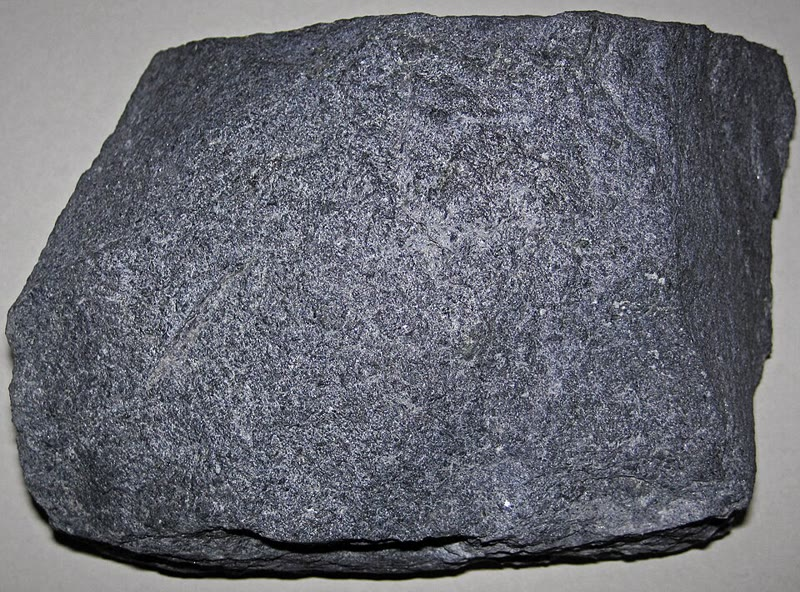
\includegraphics[height=4.4cm]{images/book2/g11-stjohn-blueschist.jpg}\hspace{0.03\linewidth}%
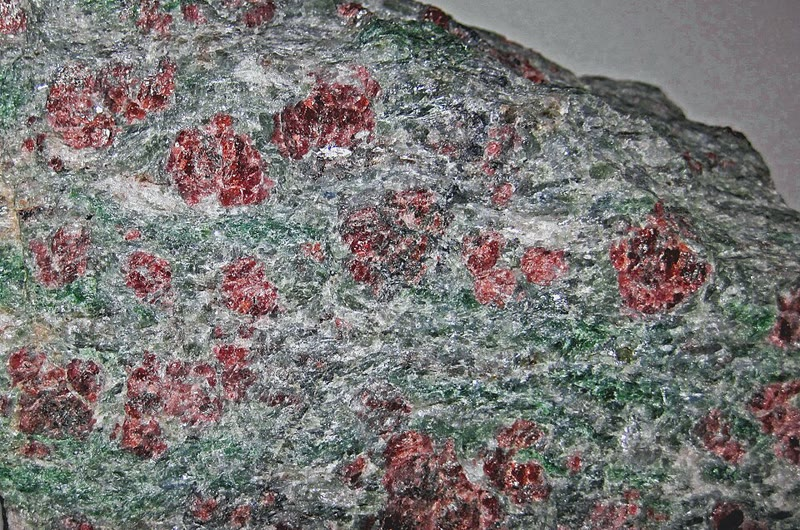
\includegraphics[height=4.4cm]{images/book2/g11-stjohn-eclogite.jpg}

{\small في اليمين: \omterm{def:g11:subduction-zones:eclogite}{شيست أزرق} من جزيرة سانتا كاتالينا، في كاليفورنيا، كان \omterm{def:g11:ocean-ridges:oceanic-lithosphere}{قشرة
محيطية} دُفنت في \omterm{def:g11:subduction-zones:subduction}{نطاق اندساس}. في اليسار: \omterm{def:g11:subduction-zones:eclogite}{إكلوجيت} من النرويج، فيه بلورات عقيق
حمراء في بيروكسين أخضر. الصورتان: جيمس سانت~جون (\babelsublr{CC~BY~2.0}).}
\end{omfigure}
% ledger: photo:g11-blueschist, photo:g11-eclogite

\omterm{def:g11:subduction-zones:eclogite}{الإكلوجيت} أكثف من البازلت؛ بل هو أكثف من \omterm{def:g11:ocean-ridges:peridotite}{بيريدوتيت}
الوشاح، بنحو \qty{6}{\percent}. فما إن تتحول قشرة \omterm{def:g11:subduction-zones:slab}{اللوح} إلى \omterm{def:g11:subduction-zones:eclogite}{إكلوجيت} حتى
لا يعود يحمل طبقة خفيفة في أعلاه: فيصير \omterm{def:g11:subduction-zones:slab}{اللوح} كله أكثف
من الوشاح المحيط به، ويشد بقوة أكبر. والصخور من هذا النوع، التي أعادتها
إلى السطح حركات لاحقة، من الشواهد المباشرة القليلة على
ما يجري على عمق عشرات الكيلومترات في \omterm{def:g11:subduction-zones:subduction}{نطاق اندساس}.
% ledger: hacker03:eclogite, photo:g11-eclogite

\begin{omfigure}
\begin{tikzpicture}[font=\footnotesize, scale=0.85]
  % subduction zone, a drawing, not to scale: slab top flat to x = -1, then bends to a 42-degree dip
  % coordinates computed once by a small script (scratch, not kept): slab top flat to x=-1, arc R=3 to a 42-degree dip
  \fill[omProp!10] (-7,-1.4) rectangle (7,-6.0);
  \fill[omSea!45] (-7,0) -- (-1,0) -- (1.6,0.8) -- (-7,0.8) -- cycle;
  \fill[lith peridotite] (-7.000,0.000) -- (-6.644,0.000) -- (-6.289,0.000) -- (-5.933,0.000) -- (-5.578,0.000) -- (-5.222,0.000) -- (-4.867,0.000) -- (-4.511,0.000) -- (-4.156,0.000) -- (-3.800,0.000) -- (-3.445,0.000) -- (-3.089,0.000) -- (-2.734,0.000) -- (-2.378,0.000) -- (-2.023,0.000) -- (-1.667,0.000) -- (-1.312,0.000) -- (-0.956,-0.000) -- (-0.602,-0.027) -- (-0.253,-0.094) -- (0.085,-0.203) -- (0.408,-0.351) -- (0.712,-0.536) -- (0.991,-0.756) -- (1.255,-0.994) -- (1.519,-1.232) -- (1.784,-1.470) -- (2.048,-1.707) -- (2.312,-1.945) -- (2.576,-2.183) -- (2.840,-2.421) -- (3.105,-2.659) -- (3.369,-2.897) -- (3.633,-3.135) -- (3.897,-3.373) -- (4.161,-3.611) -- (4.426,-3.848) -- (4.690,-4.086) -- (4.954,-4.324) -- (5.218,-4.562) -- (5.483,-4.800) -- (4.546,-5.840) -- (4.282,-5.603) -- (4.017,-5.365) -- (3.753,-5.127) -- (3.489,-4.889) -- (3.225,-4.651) -- (2.961,-4.413) -- (2.696,-4.175) -- (2.432,-3.937) -- (2.168,-3.699) -- (1.904,-3.461) -- (1.639,-3.224) -- (1.375,-2.986) -- (1.111,-2.748) -- (0.847,-2.510) -- (0.583,-2.272) -- (0.318,-2.034) -- (0.062,-1.803) -- (-0.087,-1.686) -- (-0.249,-1.587) -- (-0.421,-1.508) -- (-0.602,-1.450) -- (-0.788,-1.414) -- (-0.977,-1.400) -- (-1.312,-1.400) -- (-1.667,-1.400) -- (-2.023,-1.400) -- (-2.378,-1.400) -- (-2.734,-1.400) -- (-3.089,-1.400) -- (-3.445,-1.400) -- (-3.800,-1.400) -- (-4.156,-1.400) -- (-4.511,-1.400) -- (-4.867,-1.400) -- (-5.222,-1.400) -- (-5.578,-1.400) -- (-5.933,-1.400) -- (-6.289,-1.400) -- (-6.644,-1.400) -- (-7.000,-1.400) -- cycle;
  \fill[lith basalt] (-7.000,0.000) -- (-6.644,0.000) -- (-6.289,0.000) -- (-5.933,0.000) -- (-5.578,0.000) -- (-5.222,0.000) -- (-4.867,0.000) -- (-4.511,0.000) -- (-4.156,0.000) -- (-3.800,0.000) -- (-3.445,0.000) -- (-3.089,0.000) -- (-2.734,0.000) -- (-2.378,0.000) -- (-2.023,0.000) -- (-1.667,0.000) -- (-1.312,0.000) -- (-0.956,-0.000) -- (-0.602,-0.027) -- (-0.253,-0.094) -- (0.085,-0.203) -- (0.408,-0.351) -- (0.712,-0.536) -- (0.991,-0.756) -- (1.255,-0.994) -- (1.519,-1.232) -- (1.784,-1.470) -- (2.048,-1.707) -- (2.312,-1.945) -- (2.576,-2.183) -- (2.840,-2.421) -- (3.105,-2.659) -- (3.369,-2.897) -- (3.633,-3.135) -- (3.897,-3.373) -- (4.161,-3.611) -- (4.426,-3.848) -- (4.690,-4.086) -- (4.954,-4.324) -- (5.218,-4.562) -- (5.483,-4.800) -- (5.282,-5.023) -- (5.018,-4.785) -- (4.753,-4.547) -- (4.489,-4.309) -- (4.225,-4.071) -- (3.961,-3.833) -- (3.697,-3.596) -- (3.432,-3.358) -- (3.168,-3.120) -- (2.904,-2.882) -- (2.640,-2.644) -- (2.376,-2.406) -- (2.111,-2.168) -- (1.847,-1.930) -- (1.583,-1.692) -- (1.319,-1.455) -- (1.054,-1.217) -- (0.792,-0.980) -- (0.541,-0.783) -- (0.268,-0.616) -- (-0.023,-0.483) -- (-0.328,-0.385) -- (-0.642,-0.324) -- (-0.960,-0.300) -- (-1.312,-0.300) -- (-1.667,-0.300) -- (-2.023,-0.300) -- (-2.378,-0.300) -- (-2.734,-0.300) -- (-3.089,-0.300) -- (-3.445,-0.300) -- (-3.800,-0.300) -- (-4.156,-0.300) -- (-4.511,-0.300) -- (-4.867,-0.300) -- (-5.222,-0.300) -- (-5.578,-0.300) -- (-5.933,-0.300) -- (-6.289,-0.300) -- (-6.644,-0.300) -- (-7.000,-0.300) -- cycle;
  \fill[blue!30] (2.484,-2.100) -- (2.604,-2.208) -- (2.725,-2.317) -- (2.845,-2.425) -- (2.965,-2.533) -- (3.085,-2.642) -- (3.206,-2.750) -- (3.326,-2.858) -- (3.446,-2.967) -- (3.567,-3.075) -- (3.687,-3.183) -- (3.807,-3.292) -- (3.928,-3.400) -- (3.727,-3.623) -- (3.607,-3.515) -- (3.486,-3.406) -- (3.366,-3.298) -- (3.246,-3.190) -- (3.125,-3.081) -- (3.005,-2.973) -- (2.885,-2.865) -- (2.764,-2.756) -- (2.644,-2.648) -- (2.524,-2.540) -- (2.403,-2.431) -- (2.283,-2.323) -- cycle;
  \fill[lith eclogite] (3.928,-3.400) -- (4.057,-3.517) -- (4.187,-3.633) -- (4.316,-3.750) -- (4.446,-3.867) -- (4.576,-3.983) -- (4.705,-4.100) -- (4.835,-4.217) -- (4.964,-4.333) -- (5.094,-4.450) -- (5.223,-4.567) -- (5.353,-4.683) -- (5.483,-4.800) -- (5.282,-5.023) -- (5.152,-4.906) -- (5.023,-4.790) -- (4.893,-4.673) -- (4.764,-4.556) -- (4.634,-4.440) -- (4.504,-4.323) -- (4.375,-4.206) -- (4.245,-4.090) -- (4.116,-3.973) -- (3.986,-3.856) -- (3.857,-3.740) -- (3.727,-3.623) -- cycle;
  \draw[black!60] (-7.000,0.000) -- (-6.644,0.000) -- (-6.289,0.000) -- (-5.933,0.000) -- (-5.578,0.000) -- (-5.222,0.000) -- (-4.867,0.000) -- (-4.511,0.000) -- (-4.156,0.000) -- (-3.800,0.000) -- (-3.445,0.000) -- (-3.089,0.000) -- (-2.734,0.000) -- (-2.378,0.000) -- (-2.023,0.000) -- (-1.667,0.000) -- (-1.312,0.000) -- (-0.956,-0.000) -- (-0.602,-0.027) -- (-0.253,-0.094) -- (0.085,-0.203) -- (0.408,-0.351) -- (0.712,-0.536) -- (0.991,-0.756) -- (1.255,-0.994) -- (1.519,-1.232) -- (1.784,-1.470) -- (2.048,-1.707) -- (2.312,-1.945) -- (2.576,-2.183) -- (2.840,-2.421) -- (3.105,-2.659) -- (3.369,-2.897) -- (3.633,-3.135) -- (3.897,-3.373) -- (4.161,-3.611) -- (4.426,-3.848) -- (4.690,-4.086) -- (4.954,-4.324) -- (5.218,-4.562) -- (5.483,-4.800);
  \draw[black!60] (-7.000,-1.400) -- (-6.644,-1.400) -- (-6.289,-1.400) -- (-5.933,-1.400) -- (-5.578,-1.400) -- (-5.222,-1.400) -- (-4.867,-1.400) -- (-4.511,-1.400) -- (-4.156,-1.400) -- (-3.800,-1.400) -- (-3.445,-1.400) -- (-3.089,-1.400) -- (-2.734,-1.400) -- (-2.378,-1.400) -- (-2.023,-1.400) -- (-1.667,-1.400) -- (-1.312,-1.400) -- (-0.977,-1.400) -- (-0.788,-1.414) -- (-0.602,-1.450) -- (-0.421,-1.508) -- (-0.249,-1.587) -- (-0.087,-1.686) -- (0.062,-1.803) -- (0.318,-2.034) -- (0.583,-2.272) -- (0.847,-2.510) -- (1.111,-2.748) -- (1.375,-2.986) -- (1.639,-3.224) -- (1.904,-3.461) -- (2.168,-3.699) -- (2.432,-3.937) -- (2.696,-4.175) -- (2.961,-4.413) -- (3.225,-4.651) -- (3.489,-4.889) -- (3.753,-5.127) -- (4.017,-5.365) -- (4.282,-5.603) -- (4.546,-5.840);
  \draw[black!60] (5.483,-4.800) -- (4.546,-5.840);
  \fill[omLithGranite!55] (-1.000,0.000) -- (1.600,0.800) -- (7.000,0.800) -- (7.000,-1.600) -- (1.929,-1.600) -- (1.801,-1.485) -- (1.673,-1.370) -- (1.545,-1.255) -- (1.417,-1.140) -- (1.290,-1.025) -- (1.162,-0.910) -- (1.034,-0.795) -- (0.904,-0.682) -- (0.768,-0.577) -- (0.627,-0.479) -- (0.480,-0.390) -- (0.328,-0.310) -- (0.172,-0.238) -- (0.011,-0.176) -- (-0.152,-0.122) -- (-0.318,-0.078) -- (-0.487,-0.044) -- (-0.657,-0.020) -- (-0.828,-0.005) -- (-1.000,0.000) -- cycle;
  \fill[omLithAlluv] (-1.000,0.000) -- (0.550,0.470) -- (0.926,-0.700) -- (0.761,-0.571) -- (0.588,-0.455) -- (0.407,-0.350) -- (0.219,-0.259) -- (0.025,-0.180) -- (-0.174,-0.116) -- (-0.377,-0.065) -- (-0.583,-0.029) -- (-0.791,-0.007) -- (-1.000,0.000) -- cycle;
  \draw[black!60] (-1.000,0.000) -- (1.600,0.800) -- (7.000,0.800) -- (7.000,-1.600) -- (1.929,-1.600) -- (1.801,-1.485) -- (1.673,-1.370) -- (1.545,-1.255) -- (1.417,-1.140) -- (1.290,-1.025) -- (1.162,-0.910) -- (1.034,-0.795) -- (0.904,-0.682) -- (0.768,-0.577) -- (0.627,-0.479) -- (0.480,-0.390) -- (0.328,-0.310) -- (0.172,-0.238) -- (0.011,-0.176) -- (-0.152,-0.122) -- (-0.318,-0.078) -- (-0.487,-0.044) -- (-0.657,-0.020) -- (-0.828,-0.005) -- (-1.000,0.000);
  \draw[omThm!75, densely dashed, line width=0.7pt] (-7.000,-1.150) -- (-6.648,-1.150) -- (-6.296,-1.150) -- (-5.945,-1.150) -- (-5.593,-1.150) -- (-5.241,-1.150) -- (-4.889,-1.150) -- (-4.538,-1.150) -- (-4.186,-1.150) -- (-3.834,-1.150) -- (-3.482,-1.150) -- (-3.130,-1.150) -- (-2.779,-1.150) -- (-2.427,-1.150) -- (-2.075,-1.150) -- (-1.723,-1.150) -- (-1.372,-1.150) -- (-1.020,-1.150) -- (-0.796,-1.161) -- (-0.582,-1.198) -- (-0.374,-1.259) -- (-0.175,-1.344) -- (0.013,-1.452) -- (0.187,-1.581) -- (0.419,-1.788) -- (0.680,-2.023) -- (0.942,-2.259) -- (1.203,-2.494) -- (1.465,-2.730) -- (1.726,-2.965) -- (1.987,-3.200) -- (2.249,-3.436) -- (2.510,-3.671) -- (2.772,-3.907) -- (3.033,-4.142) -- (3.294,-4.377) -- (3.556,-4.613) -- (3.817,-4.848) -- (4.079,-5.083) -- (4.340,-5.319) -- (4.602,-5.554) -- (5.103,-4.997) -- (5.045,-4.944) -- (4.987,-4.892) -- (4.929,-4.839) -- (4.870,-4.787) -- (4.812,-4.734) -- (4.754,-4.682) -- (4.695,-4.629) -- (4.637,-4.577) -- (4.579,-4.524) -- (4.520,-4.472) -- (4.462,-4.419) -- (4.404,-4.367) -- (4.346,-4.315) -- (4.287,-4.262) -- (4.229,-4.210) -- (4.171,-4.157) -- (4.112,-4.105) -- (4.054,-4.052) -- (3.996,-4.000) -- (3.937,-3.947) -- (3.879,-3.895) -- (3.821,-3.842) -- (3.763,-3.790) -- (3.704,-3.737) -- (3.646,-3.685) -- (3.588,-3.632) -- (3.529,-3.580) -- (3.471,-3.527) -- (3.413,-3.475) -- (3.355,-3.422) -- (3.296,-3.370) -- (3.238,-3.317) -- (3.180,-3.265) -- (3.121,-3.212) -- (3.063,-3.160) -- (3.005,-3.107) -- (2.946,-3.055) -- (2.888,-3.002) -- (2.830,-2.950) -- (2.772,-2.897) -- (7.000,-2.897);
  \foreach \p in {(-0.72,-0.22),(-0.46,-0.36),(-0.18,-0.37),(0.05,-0.55),(0.29,-0.67),(0.63,-0.66),(0.87,-0.82),(0.91,-1.23),(1.27,-1.29),(1.50,-1.49),(1.55,-1.89),(1.90,-1.96),(2.04,-2.25),(2.35,-2.36),(2.54,-2.61),(2.88,-2.69),(2.99,-3.02),(3.16,-3.28),(3.47,-3.40),(3.65,-3.66),(3.89,-3.84),(4.26,-3.89),(4.32,-4.27),(4.59,-4.43),(4.88,-4.56),(5.17,-4.70)} \fill[black] \p circle (1.3pt);
  % volcanic arc above the slab, back-arc stretched
  \fill[black!70] (3.35,0.8) -- (3.7,1.4) -- (4.05,0.8) -- cycle;
  \draw[black!45, dashed] (5.2,0.8) -- (5.2,-1.6); \draw[black!45, dashed] (6.6,0.8) -- (6.6,-1.6);
  \draw[{Stealth[length=4pt]}-{Stealth[length=4pt]}, black!70] (5.35,-0.7) -- (6.45,-0.7);
  % motion arrows
  \draw[-{Stealth[length=5pt]}, line width=1pt] (-5.6,0.4) -- (-3.6,0.4);
  \draw[-{Stealth[length=5pt]}, line width=1pt] (1.77,-4.01) -- (2.88,-5.01);
  % labels
  \draw[black!60] (-1.0,0.02) -- (-1.8,1.05);
  \node[anchor=south] at (-1.8,1.05) {الخندق};
  \draw[black!60] (0.1,0.12) -- (0.5,1.05);
  \node[anchor=south, align=center] at (0.6,1.05) {رواسب\\مكشوطة};
  \node[anchor=south] at (2.35,0.85) {مقدمة القوس};
  \node[anchor=south] at (3.7,1.4) {القوس البركاني};
  \node[anchor=south] at (5.9,0.85) {ما وراء القوس};
  \node[anchor=south] at (-5.4,0.82) {قاع المحيط يتحرك نحو الخندق};
  \draw[black!60] (-7.0,-0.15) -- (-7.25,-0.15);
  \node[anchor=east] at (-7.25,-0.15) {القشرة المحيطية};
  \draw[black!60] (-7.0,-0.85) -- (-7.25,-0.85);
  \node[anchor=east, align=right] at (-7.25,-0.85) {الجزء الوشاحي\\من الغلاف الصخري};
  \node at (-3.5,-3.6) {الغلاف اللدن};
  \node[rotate=-42] at (3.98,-4.46) {اللوح المندس};
  \draw[black!60] (3.35,-2.65) -- (4.3,-2.35);
  \node[anchor=west] at (4.3,-2.35) {الشيست الأزرق};
  \draw[black!60] (5.1,-4.3) -- (5.75,-4.6);
  \node[anchor=west] at (5.75,-4.6) {الإكلوجيت};
  \node[anchor=north east, text=omThm!80!black, align=right] at (7,-2.95) {خط تساوي\\درجة الحرارة};
  \fill[black] (-6.8,-5.55) circle (1.3pt);
  \node[anchor=west] at (-6.65,-5.55) {الزلازل};
\end{tikzpicture}

{\small \omterm{def:g11:subduction-zones:subduction}{نطاق اندساس} (رسم، ليس بمقياس رسم حقيقي). ينثني \omterm{def:g11:ocean-ridges:oceanic-lithosphere}{الغلاف الصخري المحيطي} القديم
نحو الأسفل عند الخندق ويغوص تحت الصفيحة الراكبة. والرواسب
المكشوطة عن سطحه تتراكم على حافة الصفيحة الراكبة؛
والزلازل تتبع \omterm{def:g11:subduction-zones:slab}{اللوح} الغائص؛ وقشرته تتحول إلى \omterm{def:g11:subduction-zones:eclogite}{شيست أزرق}، ثم
إلى \omterm{def:g11:subduction-zones:eclogite}{إكلوجيت}. ويبقى \omterm{def:g11:subduction-zones:slab}{اللوح} أبرد من الوشاح المحيط به: فخطوط
تساوي درجة الحرارة تنجرّ نحو الأسفل على امتداده. وخط من البراكين،
القوس البركاني، يقوم فوق \omterm{def:g11:subduction-zones:slab}{اللوح}.}
\end{omfigure}
% volcanic arc above the slab: told only, defined and sourced in g12.04

\section{تشريح نطاق الاندساس}

من المحيط إلى القارة، أو إلى المحيط التالي، \omterm{def:g11:subduction-zones:subduction}{لنطاق الاندساس}
دائمًا الأجزاء نفسها.

\begin{itemize}
  \item \emph{الخندق}، حيث تنثني الصفيحة الغائصة نحو الأسفل: وهو أعمق
        مواضع المحيطات.
  \item \emph{مقدمة القوس}، بين الخندق وخط البراكين. وحافتها
        كومة من الرواسب المكشوطة عن الصفيحة الغائصة؛ وتحتها
        تنزلق الصفيحتان إحداهما على الأخرى على امتداد الحد بين الصفيحتين، وهو
        صدع لطيف الميل تحدث عليه الزلازل الكبرى، مثل
        زلزال 2011 قبالة اليابان (المثال أدناه).
  \item \emph{القوس البركاني}، خط من البراكين موازٍ للخندق،
        على جزر (تونغا وجزر ماريانا واليابان) أو على قارة (الأنديز)؛
        وسبب تكوّنه موضوع \cref{ch:g12:subduction-magmatism}.
  \item خلف بعض الأقواس، منطقة \emph{ما وراء القوس}، حيث تتمطط الصفيحة
        الراكبة؛ وخلف تونغا تتعرض للانشقاق.
\end{itemize}
% ledger: bevis95:tonga (back-arc extension at Tonga); usgs:tohoku (largest earthquakes on the
% plate boundary: example below)

خلف تونغا يحمل تمطط منطقة ما وراء القوس القوسَ نفسه نحو
الصفيحة الهادئة، كما بيّن تحديد المواقع بالأقمار الصناعية. لذلك فإن المعدل الذي يتقارب به جانبا خندق تونغا
أكبر من سرعة أي من الصفيحتين وحدها: فبحسب النموذج PB2002،
يبلغ نحو \qty{17}{cm} في السنة قرب \ang{20} جنوبًا.
% values: tonga_rate 168.0 (mean of the PB2002 TO/PA steps within 100 km of the profile);
% PB2002 steps along Tonga: 104 to 237 mm/yr; ledger data:pb2002, bevis95:tonga

\begin{example}[زلزال توهوكو، 2011]\label{ex:g11:subduction-zones:tohoku}
في 11~مارس 2011 ضرب زلزال قدره 9.1 قبالة الساحل الشمالي الشرقي
لجزيرة هونشو، في اليابان. ووقع على عمق نحو \qty{25}{km}، على الحد بين
الصفيحتين نفسه، حيث تغوص الصفيحة الهادئة، المتحركة غربًا بنحو \qty{83}{mm} في
السنة بالنسبة إلى الصفيحة التي تحمل شمال اليابان، تحتها عند
خندق اليابان. وانزلق جانبا الصدع أحدهما بالنسبة إلى الآخر بمقدار
يصل إلى 50 أو \qty{60}{m}، على مساحة طولها نحو \qty{400}{km}
وعرضها \qty{150}{km}. وتحرك قاع البحر الذي فوقها معها، فولّد تسونامي
بلغ ارتفاعه على الساحل \qty{38}{m}؛ وقُتل ما لا يقل عن \num{15703} شخصًا
وفُقد \num{4647}. وكان الساحل نفسه قد ضربته
موجات تسونامي آتية من \omterm{def:g11:subduction-zones:subduction}{نطاق الاندساس} هذا في 1611 و1896 و1933، وربما ضربه تسونامي
بحجم تسونامي 2011 عام 869.
\end{example}
% ledger: usgs:tohoku

\begin{omfigure}
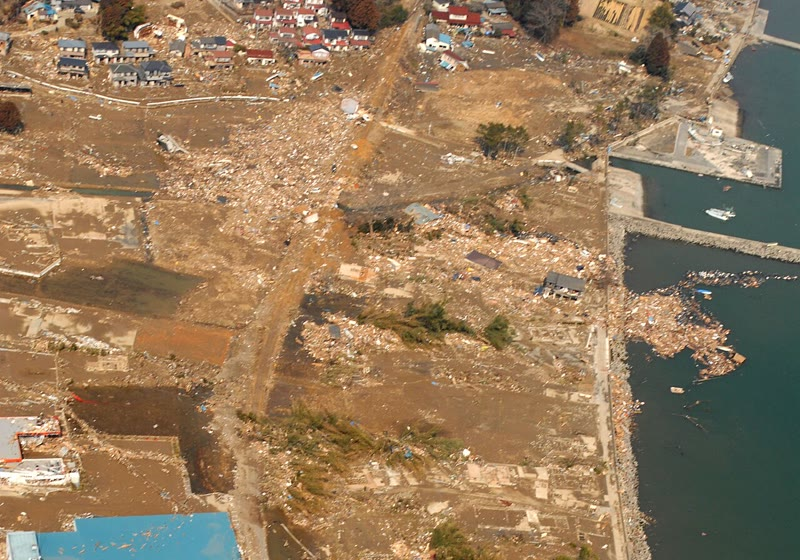
\includegraphics[width=0.78\linewidth]{images/book2/g11-usn-tsunami-kesennuma.jpg}

{\small ميناء الصيد في كيسينوما، على الساحل الشمالي الشرقي لليابان، بعد
يومين من تسونامي 11~مارس 2011. الصورة: ديلان ماكورد، البحرية الأمريكية
(ملك عام).}
\end{omfigure}
% ledger: photo:g11-tsunami

\section{تمارين}

\begin{exercise}[$\star$]\label{exo:g11:subduction-zones:1}
عرّف \omterm{def:g11:subduction-zones:subduction}{الاندساس} \omterm{def:g11:subduction-zones:subduction}{ونطاق الاندساس}. أي نوع من \omterm{def:g11:lithosphere-asthenosphere:lithosphere}{الغلاف الصخري} يغوص عند
\omterm{def:g11:subduction-zones:subduction}{نطاق اندساس}، ولماذا هذا النوع؟
\end{exercise}

\begin{exercise}[$\star$]\label{exo:g11:subduction-zones:2}
باستعمال خريطة العالم للزلازل بحسب العمق: (1) سمّ ثلاث مناطق فيها
زلازل أعمق من \qty{300}{km}؛ (2) على أي جانب من الخندق تقع
الزلازل العميقة؟ (3) وعلى امتداد ظهرة وسط الأطلسي، ما عمق
الزلازل؟
\end{exercise}

\begin{exercise}[$\star$]\label{exo:g11:subduction-zones:3}
يضم الفهرس \num{7031} زلزالًا قدرها 6 فأكثر، منها
\qty{21}{\percent} أعمق من \qty{70}{km} و\qty{6.9}{\percent} أعمق
من \qty{300}{km}. فكم زلزالًا يمثّل ذلك في كل حالة؟
\end{exercise}

\begin{exercise}[$\star$]\label{exo:g11:subduction-zones:4}
عرّف \omterm{def:g11:subduction-zones:eclogite}{الشيست الأزرق} \omterm{def:g11:subduction-zones:eclogite}{والإكلوجيت}. ما الذي يشتركان فيه مع بازلت
\omterm{def:g11:ocean-ridges:oceanic-lithosphere}{القشرة المحيطية}؟ وما الذي يختلف؟
\end{exercise}

\begin{exercise}[$\star$]\label{exo:g11:subduction-zones:5}
عدّد أجزاء \omterm{def:g11:subduction-zones:subduction}{نطاق الاندساس} بالترتيب، من قاع المحيط الذي
يتحرك نحو الخندق إلى ما وراء القوس، قائلًا في سطر واحد ما يحدث في
كل منها.
\end{exercise}

\begin{exercise}[$\star\star$]\label{exo:g11:subduction-zones:6}
في مقطع الأنديز، يمر الخط الذي يتبع الزلازل على عمق
\qty{135}{km} عند \qty{300}{km} من الخندق وعلى عمق \qty{508}{km} عند
\qty{800}{km}. احسب ميل \omterm{def:g11:subduction-zones:slab}{اللوح المندس}.
\end{exercise}

\begin{exercise}[$\star\star$]\label{exo:g11:subduction-zones:7}
\omterm{def:g11:subduction-zones:slab}{لوح مندس} مستقيم يبدأ عند خندق ويميل بزاوية \ang{45}. (1) ما عمقه على بعد
\qty{300}{km} من الخندق؟ (2) على أي بعد من الخندق
يبلغ \qty{670}{km}؟ (3) ما طول \omterm{def:g11:subduction-zones:slab}{اللوح} الواقع بين الخندق
وعمق \qty{670}{km}؟
\end{exercise}

\begin{exercise}[$\star\star$]\label{exo:g11:subduction-zones:8}
متوسطات سرعات الصفائح، بالمليمترات في السنة: كوكوس 74.6، ونازكا
70.0، والهادئة 65.5، وأستراليا 63.1، وبحر الفلبين 52.6 (ذات \omterm{def:g11:subduction-zones:slab}{ألواح})؛ والعربية
47.6، والصومال 31.0، والنوبية 29.2، وأوراسيا 22.8، وأمريكا الشمالية 19.8، والقارة القطبية الجنوبية
15.2، والكاريبي 14.9، وأمريكا الجنوبية 10.6 (بلا \omterm{def:g11:subduction-zones:slab}{ألواح}). (1) احسب متوسط
كل مجموعة والنسبة بينهما. (2) علامَ يدل هذا بشأن القوة التي
تحرّك الصفائح؟
\end{exercise}

\begin{exercise}[$\star\star$]\label{exo:g11:subduction-zones:9}
في عام 2011 انزلق الصدع قبالة اليابان بمقدار يصل إلى 50 أو \qty{60}{m}.
وتقترب الصفيحة الهادئة بمعدل \qty{83}{mm} في السنة. (1) كم سنة من حركة الصفيحة
يمثّل انزلاق قدره \qty{50}{m}، ثم \qty{60}{m}؟ (2) قارن
بالزمن المنقضي منذ عام 869، تاريخ زلزال سابق محتمل بالحجم نفسه.
\end{exercise}

\begin{exercise}[$\star\star$]\label{exo:g11:subduction-zones:10}
عمر قاع المحيط الذي يبلغ خندق اليابان نحو 133 مليون سنة،
والذي يبلغ تونغا نحو 99 والذي يبلغ الأنديز نحو 49. (1) باستعمال
قانوني \cref{ch:g11:ocean-ridges} ($2500 + 350\sqrt{t}$ حين
$t \le 70$، و$6400 - 3200\,e^{-t/62.8}$ فيما بعد)، جد عمق كل منها. (2)
أي \omterm{def:g11:lithosphere-asthenosphere:lithosphere}{غلاف صخري} هو الأبرد والأكثف؟
\end{exercise}

\begin{exercise}[$\star\star$]\label{exo:g11:subduction-zones:11}
كثافة بازلت \omterm{def:g11:ocean-ridges:oceanic-lithosphere}{القشرة المحيطية} نحو \qty{2900}{kg/m^3}،
وكثافة الوشاح المحيط \omterm{def:g11:subduction-zones:slab}{باللوح} \qty{3380}{kg/m^3}، \omterm{def:g11:subduction-zones:eclogite}{والإكلوجيت} أكثف من الوشاح
بمقدار \qty{6}{\percent}. (1) جد كثافة \omterm{def:g11:subduction-zones:eclogite}{الإكلوجيت}.
(2) بأي نسبة مئوية ترتفع كثافة القشرة حين تتحول إلى
\omterm{def:g11:subduction-zones:eclogite}{إكلوجيت}؟ (3) قبل التحول وبعده، هل القشرة أخف من الوشاح أم أكثف منه، وبكم؟
\end{exercise}

\begin{exercise}[$\star\star\star$]\label{exo:g11:subduction-zones:12}
تنتشر الحرارة بالتوصيل على مسافة قدرها نحو $\sqrt{\kappa t}$ في
زمن $t$، حيث $\kappa = \qty{1e-6}{m^2/s}$ للصخر. (1) احسب هذه المسافة
لستة ملايين سنة ($1~\text{سنة} \approx \qty{3.16e7}{s}$). (2) قارنها
بسمك \omterm{def:g11:subduction-zones:slab}{لوح مندس}، نحو \qty{100}{km}. (3) فسّر لماذا
يمكن أن تحدث زلازل داخل \omterm{def:g11:subduction-zones:slab}{لوح مندس} على عمق \qty{600}{km} بينما ينساب الوشاح المحيط
به.
\end{exercise}
% ledger: england:kelvin (kappa 1e-6 m2/s)

\begin{exercise}[$\star\star\star$]\label{exo:g11:subduction-zones:13}
تحت الأنديز عند \ang{21} جنوبًا، يبلغ خط المقطع عمق
\qty{670}{km} على بعد \qty{1017}{km} من الخندق، وتتقارب الصفيحتان بمعدل
\qty{64}{mm} في السنة. (1) قدّر طول \omterm{def:g11:subduction-zones:slab}{اللوح المندس} من الخندق حتى عمق
\qty{670}{km}. (2) كم تستغرق قطعة من قاع المحيط لتبلغ
\qty{670}{km}؟ (3) قارن بتونغا، حيث تستغرق الرحلة نفسها نحو 6
ملايين سنة.
\end{exercise}

\begin{exercise}[$\star\star\star$]\label{exo:g11:subduction-zones:14}
خذ \omterm{def:g11:subduction-zones:slab}{لوحًا مندسًا} سمكه \qty{100}{km}، أكثف من الوشاح المحيط به بمقدار
\qty{36}{kg/m^3} في المتوسط، وطوله \qty{1000}{km}، تحت خندق.
(1) احسب فائض كتلة \omterm{def:g11:subduction-zones:slab}{اللوح} لكل متر من الخندق. (2) احسب
وزنه، مع $g = \qty{9.8}{m/s^2}$. (3) لماذا تستطيع هذه القوة أن تجذب الصفيحة
كلها؟
\end{exercise}

\begin{exercise}[$\star\star\star$]\label{exo:g11:subduction-zones:15}
على امتداد خندق تونغا يعطي النموذج PB2002 تقاربًا قدره
\qty{104}{mm} في السنة عند \ang{23.6} جنوبًا و\qty{237}{mm} في السنة عند
\ang{16.5} جنوبًا. (1) ما المسافة بين النقطتين، على امتداد خط زوال
($\ang{1} \approx \qty{111}{km}$)؟ (2) بكم يزداد المعدل لكل
مئة كيلومتر؟ (3) تتحرك الصفيحة الهادئة بالسرعة نفسها تقريبًا عند
النقطتين. فماذا يجب أن يفعل الجانب الآخر من الخندق، قوس تونغا؟
\end{exercise}

\section{مسألة: لوح تونغا المندس}

\begin{problem}[{مسألة نهاية الأسبوع --- من الخندق إلى \qty{670}{km}}]
\label{pb:g11:subduction-zones:1}
% values: tonga fit -23.568 + 0.91068 x; tonga_rate 168.0 mm/yr; tonga_age 98.8;
% x670 761.6; path 1014; time 6.04 Myr; tonga_maxdepth 670.8 (slab_sections.py);
% MKEA 69 mm/yr (plate_velocities.py); kappa england:kelvin; eclogite hacker03:eclogite
تحت خندق تونغا تغوص الصفيحة الهادئة نحو الغرب. استعمل مقطع
تونغا في هذا الفصل، ومعادلة خطه $z = -24 + 0.91\,x$ (كلاهما
بالكيلومترات، و$x$ مقيس من الخندق نحو القوس).

\medskip
\noindent\textbf{الجزء الأول --- المقطع الزلزالي.}
\begin{enumerate}
  \item ما عمق أعمق زلزال في المقطع؟
  \item لماذا لا توجد زلازل عميقة على الجانب المحيطي من الخندق؟
  \item احسب عمق الخط عند $x = 300$ و$x = 700$، ثم
        ميل \omterm{def:g11:subduction-zones:slab}{اللوح المندس}.
  \item على أي بعد أفقي من الخندق يكون عمق \omterm{def:g11:subduction-zones:slab}{اللوح}
        \qty{100}{km}؟ و\qty{400}{km}؟
  \item يمر الخط على ارتفاع \qty{24}{km} فوق الخندق عند $x = 0$. فماذا
        يخبرك هذا عن شكل \omterm{def:g11:subduction-zones:slab}{اللوح} قرب الخندق؟
\end{enumerate}

\medskip
\noindent\textbf{الجزء الثاني --- التقارب.}
\begin{enumerate}[resume]
  \item تتقارب الصفيحتان عبر الخندق بنحو \qty{168}{mm} في السنة.
        حوّل ذلك إلى سنتيمترات في السنة وإلى كيلومترات في كل مليون سنة.
  \item تتحرك الصفيحة الهادئة فوق هاواي بنحو \qty{69}{mm} في السنة.
        فكم مرة يكون التقارب عند تونغا أسرع؟
  \item باستعمال جمع السرعات النسبية، فسّر كيف يمكن للتقارب أن
        يتجاوز سرعة الصفيحة الهادئة.
  \item عمر القاع الذي يبلغ الخندق نحو 99 مليون سنة. فعلى أي
        عمق يقع (القانون الأسي في \cref{ch:g11:ocean-ridges})؟
  \item لماذا يستطيع \omterm{def:g11:lithosphere-asthenosphere:lithosphere}{غلاف صخري} كهذا أن يغوص من تلقاء نفسه؟
\end{enumerate}

\medskip
\noindent\textbf{الجزء الثالث --- نزولًا حتى \qty{670}{km}.}
\begin{enumerate}[resume]
  \item على أي بعد أفقي من الخندق يبلغ الخط
        \qty{670}{km}؟
  \item قدّر طول \omterm{def:g11:subduction-zones:slab}{اللوح المندس} من الخندق حتى تلك النقطة،
        معتبرًا إياه مستقيمًا.
  \item كم تستغرق قطعة من قاع المحيط لتقطع هذا الطول بمعدل
        \qty{168}{mm} في السنة؟
  \item وكم كانت ستستغرق بمعدل \qty{69}{mm} في السنة، وهو سرعة الصفيحة
        الهادئة فوق هاواي؟
  \item في الطريق تتحول قشرة \omterm{def:g11:subduction-zones:slab}{اللوح} إلى \omterm{def:g11:subduction-zones:eclogite}{إكلوجيت}،
        أكثف بمقدار \qty{6}{\percent} من الوشاح الذي كثافته \qty{3380}{kg/m^3}. فما
        كثافته، وماذا يغيّر هذا بالنسبة إلى \omterm{def:g11:subduction-zones:slab}{اللوح}؟
\end{enumerate}

\medskip
\noindent\textbf{الجزء الرابع --- لوح بارد في وشاح ساخن.}
\begin{enumerate}[resume]
  \item خلال زمن السؤال~13، تنتشر الحرارة بالتوصيل على نحو
        $\sqrt{\kappa t}$، حيث $\kappa = \qty{1e-6}{m^2/s}$. احسب هذه
        المسافة.
  \item قارنها بسمك \omterm{def:g11:subduction-zones:slab}{اللوح}، نحو \qty{100}{km}. فهل
        يبقى \omterm{def:g11:subduction-zones:slab}{اللوح} باردًا من الداخل حين يبلغ \qty{670}{km}؟
  \item لماذا يفسّر هذا الزلازل على عمق \qty{600}{km} وأكثر
        تحت تونغا؟
  \item أي تغيّر في الوشاح كشفته الموجات الزلزالية قرب
        \qty{670}{km} (\cref{ch:g11:seismic-structure})؟
  \item استنتج: كم يستغرق قاع المحيط الهادئ لينتقل من خندق
        تونغا نزولًا حتى \qty{670}{km}؟
\end{enumerate}
\end{problem}
